% Created 2016-08-19 Fri 20:30
\documentclass[11pt]{article}
\usepackage[utf8]{inputenc}
\usepackage[T1]{fontenc}
\usepackage{fixltx2e}
\usepackage{graphicx}
\usepackage{grffile}
\usepackage{longtable}
\usepackage{wrapfig}
\usepackage{rotating}
\usepackage[normalem]{ulem}
\usepackage{amsmath}
\usepackage{textcomp}
\usepackage{amssymb}
\usepackage{capt-of}
\usepackage{hyperref}
\usepackage{xltxtra}
\usepackage{fontspec} %Font package
\usepackage{xunicode}
\setmonofont{PragmataPro}
\usepackage[top=0.25in, left=0.45in, right=0.75in, bottom=0.25in]{geometry}
\author{Nishant Gupta, nishgu@iitk.ac.in, 13447}
\date{\today}
\title{CS425 - Project 1 Report}
\hypersetup{
 pdfauthor={Nishant Gupta, nishgu@iitk.ac.in, 13447},
 pdftitle={CS425 - Project 1 Report},
 pdfkeywords={},
 pdfsubject={HTTP1.1 compliant file server},
 pdfcreator={Emacs 24.5.1 (Org mode 8.3.5)}, 
 pdflang={English}}
\begin{document}

\maketitle
\begin{center}
\texttt{\Huge HTTP File Server}
\end{center}

\section{Implemented Options}
\label{sec:orgheadline3}
\subsection{Mandatory}
\label{sec:orgheadline1}
\begin{itemize}
\item Supports GET method
\item Supports Persistent Connections and multiple clients
\item Provides Content-length and content-Type fields in response
\item Provides appropriate Status-Code and Response-Phrase values in response to errors.
\end{itemize}
\subsection{Optional}
\label{sec:orgheadline2}
\begin{itemize}
\item Allow the server port and document base directory to be initialized at start up
\item Include the Date and Server fields in the Response message header
\item Implemented the HEAD method
\item Implemented the POST method
\item Reply with a directory listing if a directory is the requested resource
\item Reply with a hyperlinked directory listing if a directory is the requested resource
\end{itemize}

\newpage
\section{Optional feature details}
\label{sec:orgheadline9}
\subsection{Server port and root directory initialization :}
\label{sec:orgheadline4}
You can optionally give port with \texttt{-p} and root with \texttt{-r}.
Default values are: \texttt{PORT=9576} and \texttt{ROOT=./}

\noindent eg: \texttt{bin/server -p 9577 -r test/}
\subsection{Date and Server fields :}
\label{sec:orgheadline5}
Server is sent as Alchemist and Date is sent in the format \texttt{Thu, 18 Aug 2016 18:52:47 GMT}.
\subsection{POST Method :}
\label{sec:orgheadline6}
In, POST request, message-body is written to \texttt{abs-path} of URI relative to root directory.
Html displaying \texttt{Content written Succesfully} is returned in response.
\noindent See Appendix
\subsection{HEAD Method :}
\label{sec:orgheadline7}
Only headers of a GET request are returned in HEAD request.

\noindent See Appendix
\subsection{Hyperlinked directory :}
\label{sec:orgheadline8}
A clickable list of all the filenames is is returned on GET request for a directory. Spaces in filenames and directories are not supported.

\newpage
\section{Test results}
\label{sec:orgheadline26}
\subsection{Multiple Clients and Persistent connections}
\label{sec:orgheadline11}
See \hyperref[sec:orgheadline10]{Multiple clients and persistent connections of Appendix} for Verification image and log.
It can be seen in chrome network inspector image that multiple requests complete at almost same time. This means that server supports multiple connections.  \\
Also Stderr log of opening \texttt{index.html} in firefox shows that multiple requests were served to same client, which proves that persistent 
connections work and the clients requests are intermingled, which proves that multiple simultaneous connections work.

\subsection{Webpage provided with project}
\label{sec:orgheadline15}
Google Chrome Version 52.0.2743.116 (64-bit) was used for testing in this part
\subsubsection{GET and Directory listing}
\label{sec:orgheadline13}
These are \hyperref[sec:orgheadline12]{Screenshots of Google Chrome} showing index.html and directory listing working correctly.

\subsubsection{POST request}
\label{sec:orgheadline14}
After submitting form on \texttt{post\_test.html}, following is the content of \texttt{test/post\_test\_file.txt}
\begin{verbatim}
TextEntry_1=Hola&TextEntry_2=This+is+some+text+for+testing+the+POST+method.%0D%0A&Item=Item_1
\end{verbatim}
\subsection{Testing using command line}
\label{sec:orgheadline21}
httpie : A CLI HTTP client was used.
\subsubsection{POST request}
\label{sec:orgheadline17}
I generated a random file of 10\(^{\text{6}}\) bytes and sent it using \texttt{httpie}, and compared the saved file to original file. They were same. 
 \hyperref[sec:orgheadline16]{POST request} section of Appendix verifies that.
\subsubsection{GET request}
\label{sec:orgheadline18}
I made a GET request using httpie and it ran succesfully as can be seen in \hyperref[sec:orgheadline12]{GET Request} section of Appendix.
\subsubsection{HEAD request}
\label{sec:orgheadline20}
I made a HEAD request using  httpie and it ran succesfully as can be seen in \hyperref[sec:orgheadline19]{HEAD request} section of Appendix.

\subsection{Status Codes}
\label{sec:orgheadline23}
I made different types of requests that would yield different status codes using httpie. They can be seen in \hyperref[sec:orgheadline22]{Status Codes} section of Appendix.
\begin{itemize}
\item I recognize \texttt{GET, HEAD, POST, PUT, OPTIONS, CONNECT, DELETE}. Only three of them are implemented, others give \texttt{501 : Not implemented}
\item If anything other than these seven comes, it is BAD request and \texttt{400 : Bad Request} is returned. Bad request is also returned if any protocol other than HTTP/1.0 or HTTP/1.1 is requested
\item I have put my entire parser in a try catch block, if parser fails I send \texttt{500 : Internal Server Error} in catch block.
\item If Parser succeeds, I process corresponding request and then \texttt{404} or \texttt{200} is sent by corresponding method.
\end{itemize}
\subsection{Date and Server fields}
\label{sec:orgheadline24}
It can be seen in any request in Appendix that Server and Appendix Headers are returned.
\subsection{Summary}
\label{sec:orgheadline25}
\begin{itemize}
\item I have not supported spaces and other special characters in resources requested, so it will give 404.
\item Also, in hyperlinked directory listing, link will be wrong if there are spaces or other special characters in the name.
\item Everything else is working as it should.
\item I had no way to check Internal Server Error.
\item All the other Status codes are working as they should.
\item Multiple clients and persistent connections are working correctly, I have not implemented timeout.
\end{itemize}
\newpage
\section{Appendix}
\label{sec:orgheadline28}
\subsection{Multiple clients and persistent connections}
\label{sec:orgheadline10}
\label{orgtarget1}
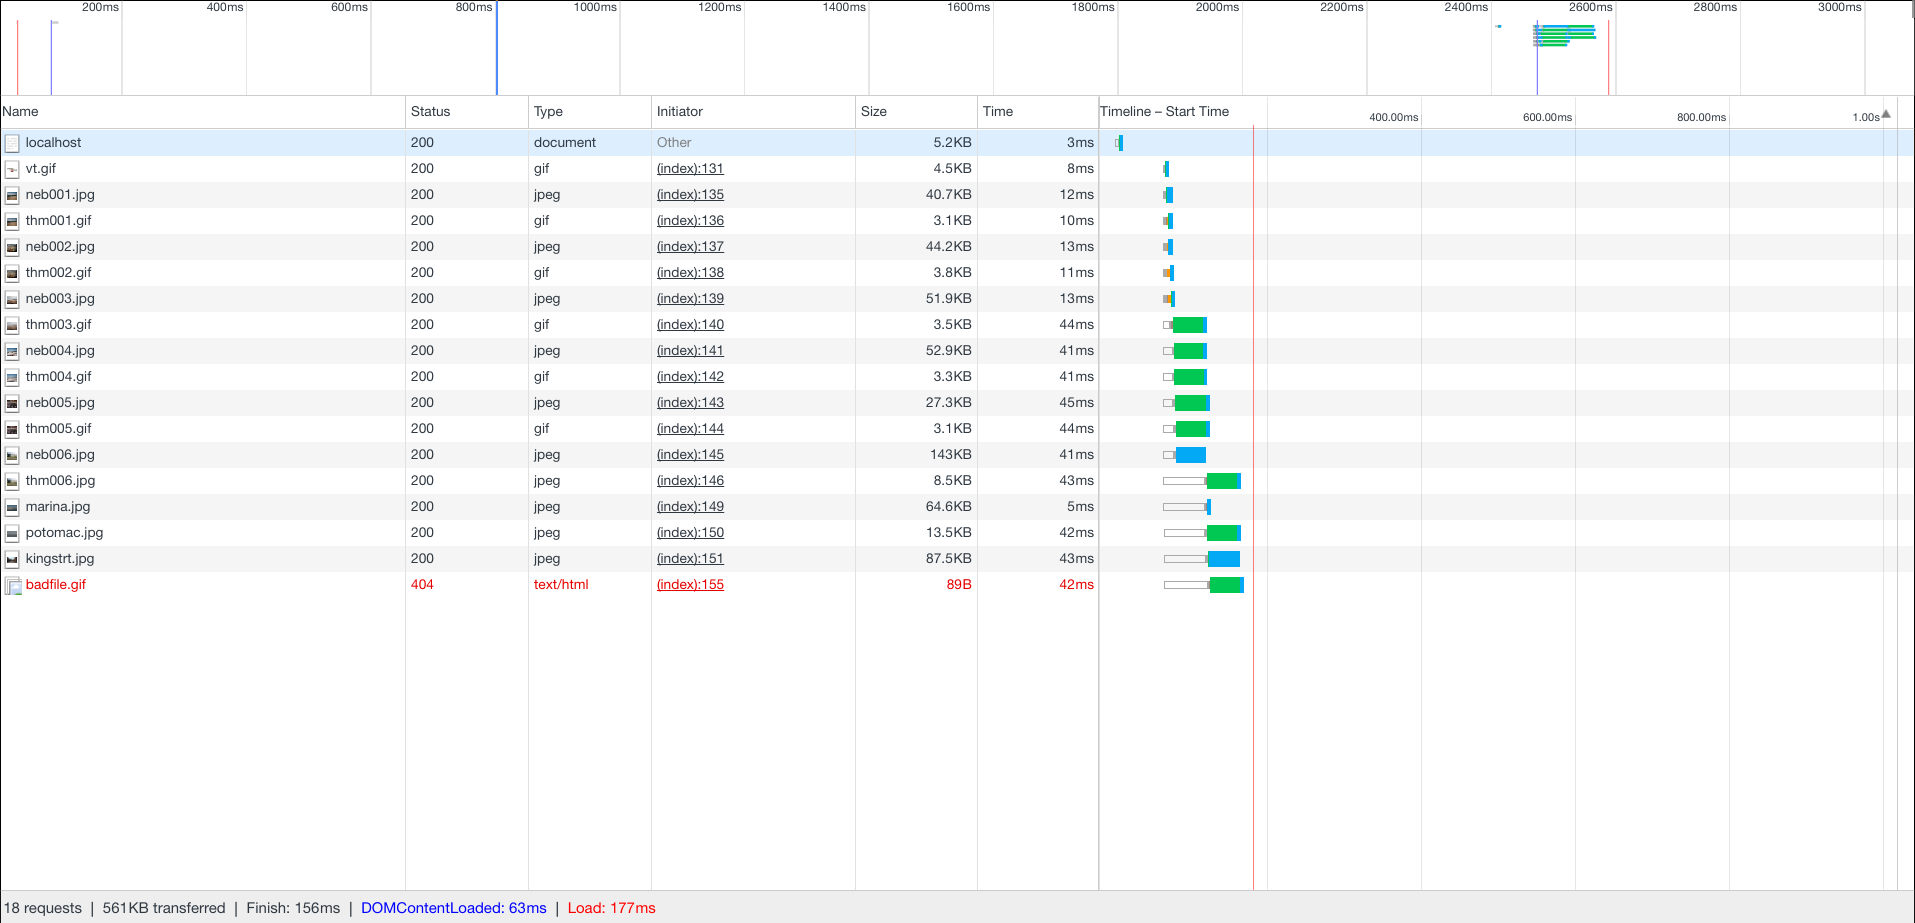
\includegraphics[width=18cm]{./multipleclients.png}


\label{orgtarget2}
\noindent Following is the condensed stderr log of opening \texttt{index.html} in firefox.

\begin{verbatim}
Connected to client 6
Request 1 from Client 5
Request 2 from Client 5
Connected to client 6
Connected to client 7
Connected to client 8
Connected to client 9
Connected to client 10
Request 1 from Client 10
Request 1 from Client 9
Request 1 from Client 8
Request 1 from Client 6
Request 1 from Client 7
Request 3 from Client 5
Request 2 from Client 8
Request 2 from Client 10
Request 2 from Client 9
Request 2 from Client 7
Request 2 from Client 6
Request 3 from Client 6
Request 4 from Client 5
Request 3 from Client 8
Request 4 from Client 6
Request 5 from Client 5
Request 5 from Client 6
Closed Client
Closed Client
Closed Client
Closed Client
Closed Client
Closed Client
\end{verbatim}

\subsection{GET Request :}
\label{sec:orgheadline12}
GET request made using Chrome

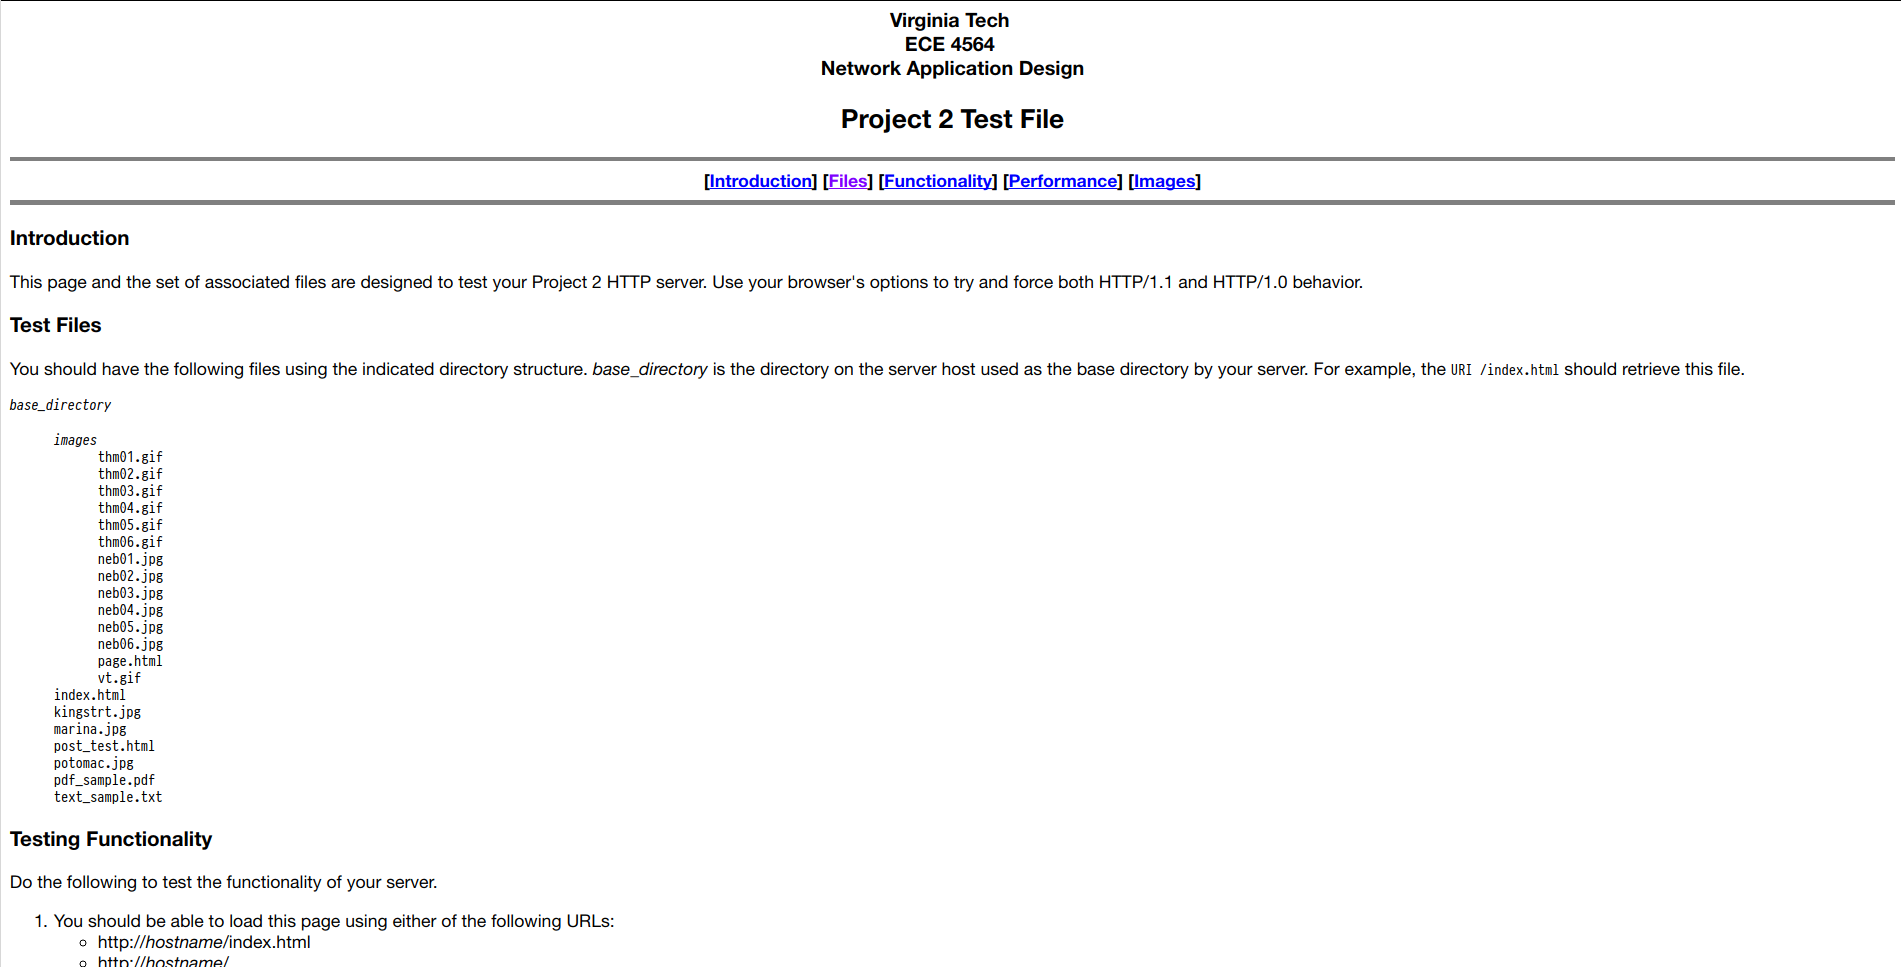
\includegraphics[width=9cm]{./index1.png}

\includegraphics[width=9cm]{./index2.png} \\

\includegraphics[width=9cm]{./directorylist.png}
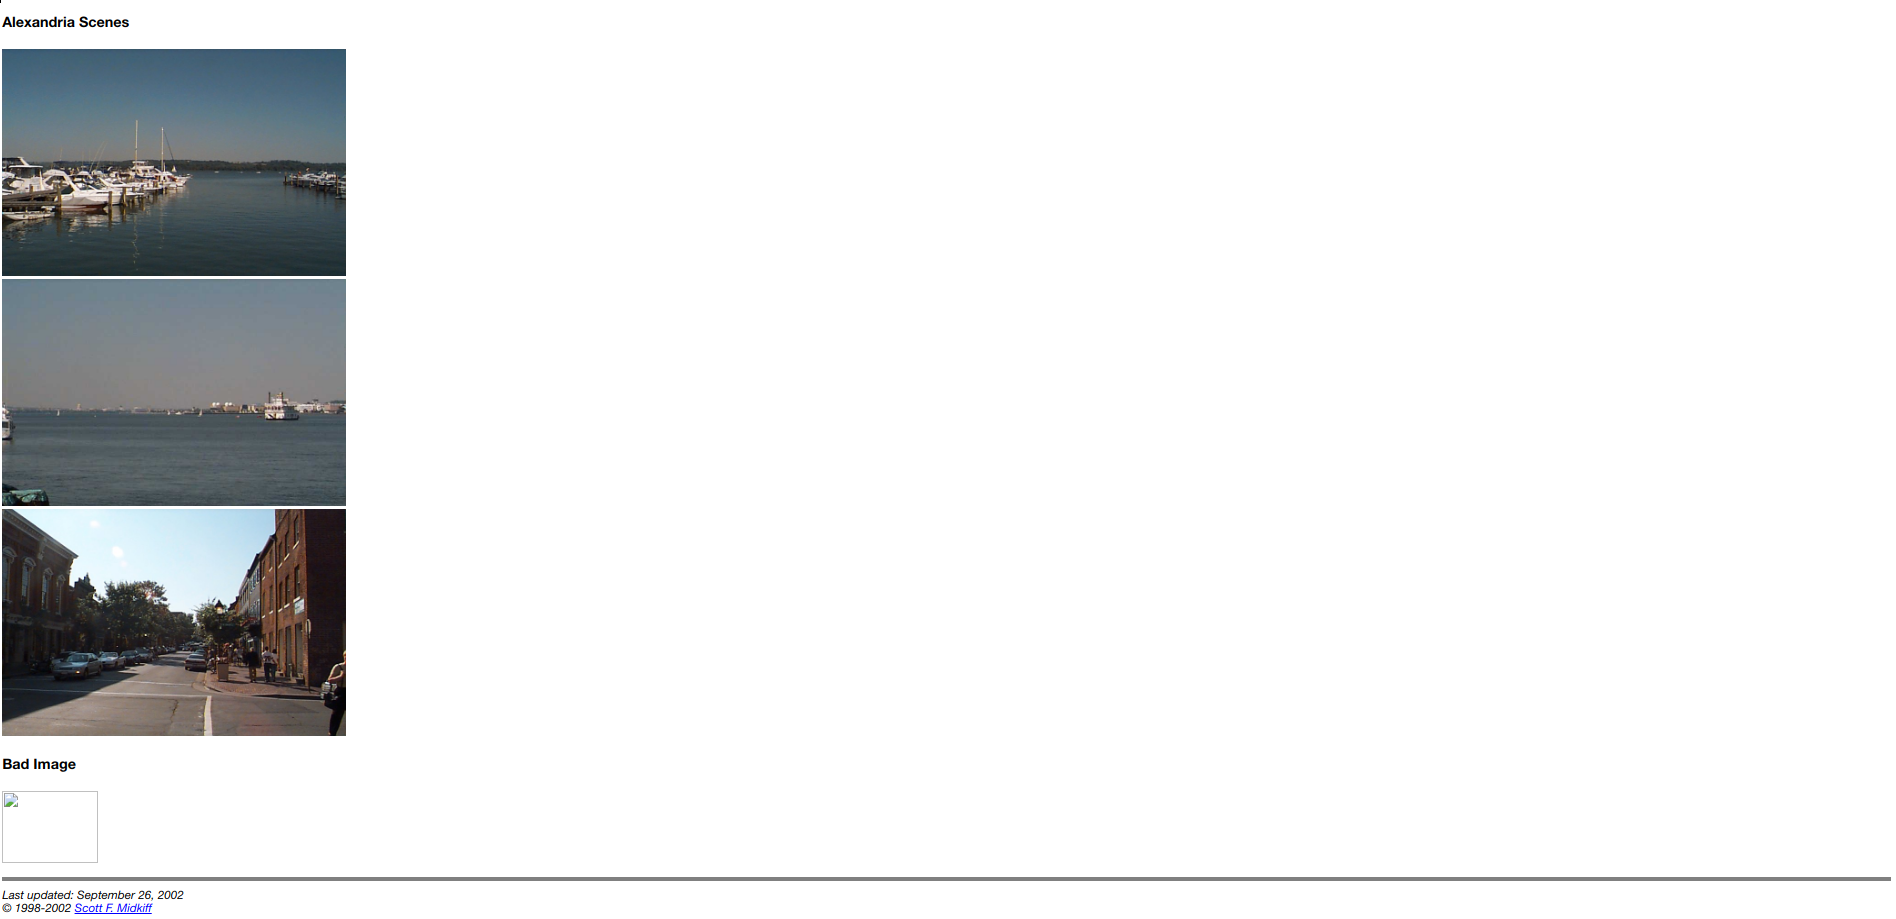
\includegraphics[width=9cm]{./index3.png}

\noindent GET request made using httpie
\begin{verbatim}
 ~/c/n/project1 $ http GET  :9577/post_test_file.txt Connection:close -v
GET /post_test_file.txt HTTP/1.1
Accept: */*
Accept-Encoding: gzip, deflate
Connection: close
Host: localhost:9577
User-Agent: HTTPie/0.9.4



HTTP/1.1 200 OK
Connection: Close
Content-Length: 93
Content-Type: text/plain
Date: Thu, 18 Aug 2016 18:52:47 GMT
Server: Alchemist

TextEntry_1=Hola&TextEntry_2=This+is+some+text+for+testing+the+POST+method.%0D%0A&Item=Item_1
\end{verbatim}

\newpage
\subsection{POST request :}
\label{sec:orgheadline16}
\label{orgtarget3}
\noindent POST Request made using httpie 

\begin{verbatim}
 ~/c/n/project1 $ base64 /dev/urandom | head -c 1000000 >! file.txt
 ~/c/n/project1 $ cat file.txt | http POST :9577/file.txt -p=Hhb
POST /file.txt HTTP/1.1
Accept: application/json
Accept-Encoding: gzip, deflate
Connection: keep-alive
Content-Length: 1000000
Content-Type: application/json
Host: localhost:9577
User-Agent: HTTPie/0.9.4

HTTP/1.1 200 OK
Connection: keep-alive 
Content-Length: 36
Content-Type: text/html
Date: Fri, 19 Aug 2016 13:31:22 GMT
Server: Alchemist

<h1>Content written Succesfully</h1>

 ~/c/n/project1 $ diff file.txt test/file.txt
 ~/c/n/project1 $
\end{verbatim}

\subsection{HEAD request :}
\label{sec:orgheadline19}
\label{orgtarget4}
HEAD request made using httpie
\begin{verbatim}
 ~/c/n/project1 $ http HEAD  :9577/ Connection:close -v
HEAD / HTTP/1.1
Accept: */*
Accept-Encoding: gzip, deflate
Connection: close
Host: localhost:9577
User-Agent: HTTPie/0.9.4



HTTP/1.1 200 OK
Connection: Close
Content-Length: 5211
Content-Type: text/html
Date: Thu, 18 Aug 2016 18:57:32 GMT
Server: Alchemist
\end{verbatim}

\newpage
\subsection{Status Codes :}
\label{sec:orgheadline22}

Following are some of httpie requests that showcase diffrent status codes
\begin{itemize}
\item Not Implemented
\end{itemize}
\begin{verbatim}
 ~/c/n/project1 $ http PUT  :9577/fajlsdfj -v
PUT /fajlsdfj HTTP/1.1
Accept: */*
Accept-Encoding: gzip, deflate
Connection: keep-alive
Content-Length: 0
Host: localhost:9577
User-Agent: HTTPie/0.9.4


HTTP/1.0 501 Not Implemented
Connection: keep-alive
Content-Length: 29
Content-Type: text/html
Date: Fri, 19 Aug 2016 13:30:57 GMT
Server: Alchemist

<h1>501: Not Implemented</h1>
\end{verbatim}
\begin{itemize}
\item Bad Request
\end{itemize}
\begin{verbatim}
 ~/c/n/project1 $ http PUT  :9577/fajlsdfj -v
PUT /fajlsdfj HTTP/1.1
Accept: */*
Accept-Encoding: gzip, deflate
Connection: keep-alive
Content-Length: 0
Host: localhost:9577
User-Agent: HTTPie/0.9.4


HTTP/1.0 501 Not Implemented
Connection: keep-alive
Content-Length: 29
Content-Type: text/html
Date: Fri, 19 Aug 2016 13:30:57 GMT
Server: Alchemist

<h1>501: Not Implemented</h1>
\end{verbatim}
\begin{itemize}
\item Not Found
\end{itemize}
\begin{verbatim}
 ~/c/n/project1 $ http GET  :9577/fajlsdfj -v
GET /fajlsdfj HTTP/1.1
Accept: */*
Accept-Encoding: gzip, deflate
Connection: keep-alive
Host: localhost:9577
User-Agent: HTTPie/0.9.4


HTTP/1.0 404 Not Found
Connection: keep-alive
Content-Length: 23
Content-Type: text/html
Date: Fri, 19 Aug 2016 13:35:36 GMT
Server: Alchemist

<h1>404: Not Found</h1>
\end{verbatim}

\subsection{Source code :}
\label{sec:orgheadline27}
\begin{verbatim}
// AUTHOR: Nishant Gupta

#include <arpa/inet.h>
#include <assert.h>
#include <dirent.h>
#include <fcntl.h>
#include <netdb.h>
#include <signal.h>
#include <stdio.h>
#include <stdlib.h>
#include <string.h>
#include <sys/socket.h>
#include <sys/stat.h>
#include <sys/types.h>
#include <time.h>
#include <unistd.h>

#define CONNMAX 1000
#define BYTES 8096
#define min(a, b) (a < b) ? a : b

char *ROOT = getenv("PWD"), PORT[8];
int listenfd;

enum requestType { GET, POST, HEAD, BAD, UNIMPLEMENTED, ERROR };
void startServer(char *);
void serveClient(int);
requestType parseHeaders(char *, int &, char *, int &);
int respondHG(char *, int, requestType, int);
int respondPOST(char *, int, int, int);
int sendCommonHeaders(int, int, int, char *);
int sendNotFound(int, requestType);
char *generateDirectoryList(char *, int &);

// Parsing the command line arguments
int parseArgs(int argc, char *argv[]) {
  char c;

  while ((c = getopt(argc, argv, "p:r:")) != -1)
    switch (c) {
    case 'r':
      ROOT = (char *)malloc(strlen(optarg));
      strcpy(ROOT, optarg);
      break;
    case 'p':
      strcpy(PORT, optarg);
      break;
    default:
      fprintf(stderr, "%s [-p PORT] [-r ROOT]\n", argv[0]);
      exit(1);
    }
  return 0;
}

int main(int argc, char *argv[]) {
  struct sockaddr_in clientaddr;
  socklen_t addrlen;
  int clientSock;
  strcpy(PORT, "9576");
  parseArgs(argc, argv);

  startServer(PORT);
  printf("Server started at port no. %s with root directory as %s\n", PORT,
         ROOT);

  while (1) {
    addrlen = sizeof(clientaddr);
    clientSock = accept(listenfd, (struct sockaddr *)&clientaddr, &addrlen);
    if (clientSock < 0)
      perror("accept() error");
    else {
      if (fork() == 0) {
        serveClient(clientSock);
        exit(0);
      }
    }
  }
  return 0;
}

// starts the server, One time call
void startServer(char *port) {
  struct addrinfo hints, *res, *p;
  int on = 1;
  // taken from `man 3 getaddrinfo`
  memset(&hints, 0, sizeof(hints));
  hints.ai_family = AF_INET;
  hints.ai_socktype = SOCK_STREAM;
  hints.ai_flags = AI_PASSIVE; // to listen to all interfaces
  if (getaddrinfo(NULL, port, &hints, &res) !=
      0) { // get a list of all interfaces to which socket is bound
    perror("getaddrinfo() error");
    exit(1);
  }
  // try to listen to atleast one
  for (p = res; p != NULL; p = p->ai_next) {
    listenfd = socket(p->ai_family, p->ai_socktype, 0);
    if (listenfd == -1)
      continue;
    if (bind(listenfd, p->ai_addr, p->ai_addrlen) == 0)
      break;
  }
  freeaddrinfo(res);
  // Entire list traversed but could not bind to anyone
  if (p == NULL) {
    perror("socket() or bind()");
    exit(1);
  }

  // free the port as soon as program exits
  setsockopt(listenfd, SOL_SOCKET, SO_REUSEADDR, &on, sizeof(on));

  if (listen(listenfd, atoi(port)) != 0) {
    perror("listen() error");
    exit(1);
  }
}

//Sends headers that are common in all thre requests, currently only GET and
//HEAD use it.
int sendCommonHeaders(int clientSock, int contentLength, int keepAliveStatus,
                      char *mimeType) {
  char tempBuffer[BYTES];
  send(clientSock, "HTTP/1.1 200 OK\r\n", 17, 0);
  send(clientSock, "Server: Alchemist\r\n", 19, 0);
  char dateBuffer[BYTES];
  time_t now = time(0);
  struct tm tm = *gmtime(&now);
  strftime(dateBuffer, sizeof(dateBuffer), "%a, %d %b %Y %H:%M:%S %Z", &tm);
  snprintf(tempBuffer, sizeof(tempBuffer), "Date: %s\r\n", dateBuffer);
  send(clientSock, tempBuffer, strlen(tempBuffer), 0);
  snprintf(tempBuffer, BYTES, "Content-Length: %d\r\n", contentLength);
  send(clientSock, tempBuffer, strlen(tempBuffer), 0);
  snprintf(tempBuffer, BYTES, "Content-Type: %s\r\n", mimeType);
  send(clientSock, tempBuffer, strlen(tempBuffer), 0);
  if (keepAliveStatus == 1)
    snprintf(tempBuffer, BYTES, "Connection: Close\r\n\r\n");
  else
    snprintf(tempBuffer, BYTES, "Connection: keep-alive \r\n\r\n");
  send(clientSock, tempBuffer, strlen(tempBuffer), 0);
  return 0;
}

// Send 404 Status
int sendNotFound(int clientSock, requestType curRequest) {
  char tempBuffer[1024];
  write(clientSock, "HTTP/1.0 404 Not Found\n", 23); // FILE NOT FOUND
  send(clientSock, "Server: Alchemist\r\n", 19, 0);
  char dateBuffer[BYTES];
  time_t now = time(0);
  struct tm tm = *gmtime(&now);
  strftime(dateBuffer, sizeof(dateBuffer), "%a, %d %b %Y %H:%M:%S %Z", &tm);
  snprintf(tempBuffer, sizeof(tempBuffer), "Date: %s\r\n", dateBuffer);
  send(clientSock, tempBuffer, strlen(tempBuffer), 0);
  char *errMesg = (char *)"<h1>404: Not Found</h1>";
  snprintf(tempBuffer, BYTES, "Content-Length: %d\n", (int)strlen(errMesg));
  send(clientSock, tempBuffer, strlen(tempBuffer), 0);
  snprintf(tempBuffer, BYTES, "Content-Type: text/html\r\n");
  send(clientSock, tempBuffer, strlen(tempBuffer), 0);
  send(clientSock, "Connection: keep-alive\n\n", 24, 0);
  if (curRequest != HEAD)
    send(clientSock, errMesg, strlen(errMesg) + 1, 0);
  return 0;
}

// Send 400 Status
int sendBadRequest(int clientSock, requestType curRequest) {
  char tempBuffer[1024];
  write(clientSock, "HTTP/1.0 400 Bad Request\r\n", 26);
  send(clientSock, "Server: Alchemist\r\n", 19, 0);
  char dateBuffer[BYTES];
  time_t now = time(0);
  struct tm tm = *gmtime(&now);
  strftime(dateBuffer, sizeof(dateBuffer), "%a, %d %b %Y %H:%M:%S %Z", &tm);
  snprintf(tempBuffer, sizeof(tempBuffer), "Date: %s\r\n", dateBuffer);
  send(clientSock, tempBuffer, strlen(tempBuffer), 0);
  char *errMesg = (char *)"<h1>400: Bad Request</h1>";
  snprintf(tempBuffer, BYTES, "Content-Length: %d\n", (int)strlen(errMesg));
  send(clientSock, tempBuffer, strlen(tempBuffer), 0);
  snprintf(tempBuffer, BYTES, "Content-Type: text/html\r\n");
  send(clientSock, tempBuffer, strlen(tempBuffer), 0);
  send(clientSock, "Connection: keep-alive\r\n\r\n", 26, 0);
  if (curRequest != HEAD)
    send(clientSock, errMesg, strlen(errMesg) + 1, 0);
  return 0;
}


// Send 500 status
int sendInternalError(int clientSock, requestType curRequest) {
  char tempBuffer[1024];
  write(clientSock, "HTTP/1.0 500 Internal Server Error\r\n", 36);
  send(clientSock, "Server: Alchemist\r\n", 19, 0);
  char dateBuffer[BYTES];
  time_t now = time(0);
  struct tm tm = *gmtime(&now);
  strftime(dateBuffer, sizeof(dateBuffer), "%a, %d %b %Y %H:%M:%S %Z", &tm);
  snprintf(tempBuffer, sizeof(tempBuffer), "Date: %s\r\n", dateBuffer);
  send(clientSock, tempBuffer, strlen(tempBuffer), 0);
  char *errMesg = (char *)"<h1>500: Internal Server Error</h1>";
  snprintf(tempBuffer, BYTES, "Content-Length: %d\n", (int)strlen(errMesg));
  send(clientSock, tempBuffer, strlen(tempBuffer), 0);
  snprintf(tempBuffer, BYTES, "Content-Type: text/html\r\n");
  send(clientSock, tempBuffer, strlen(tempBuffer), 0);
  send(clientSock, "Connection: close\r\n\r\n", 26, 0);
  if (curRequest != HEAD)
    send(clientSock, errMesg, strlen(errMesg) + 1, 0);
  exit(1);
  return 0;
}


// Send 501 status
int sendNotImplemented(int clientSock, requestType curRequest) {
  char tempBuffer[1024];
  write(clientSock, "HTTP/1.0 501 Not Implemented\r\n", 30); // FILE NOT FOUND
  send(clientSock, "Server: Alchemist\r\n", 19, 0);
  char dateBuffer[BYTES];
  time_t now = time(0);
  struct tm tm = *gmtime(&now);
  strftime(dateBuffer, sizeof(dateBuffer), "%a, %d %b %Y %H:%M:%S %Z", &tm);
  snprintf(tempBuffer, sizeof(tempBuffer), "Date: %s\r\n", dateBuffer);
  send(clientSock, tempBuffer, strlen(tempBuffer), 0);
  char *errMesg = (char *)"<h1>501: Not Implemented</h1>";
  snprintf(tempBuffer, BYTES, "Content-Length: %d\n", (int)strlen(errMesg));
  send(clientSock, tempBuffer, strlen(tempBuffer), 0);
  snprintf(tempBuffer, BYTES, "Content-Type: text/html\r\n");
  send(clientSock, tempBuffer, strlen(tempBuffer), 0);
  send(clientSock, "Connection: keep-alive\r\n\r\n", 26, 0);
  if (curRequest != HEAD)
    send(clientSock, errMesg, strlen(errMesg) + 1, 0);
  return 0;
}

// generates directory listing for hyperlinked directory part
char *generateDirectoryList(char *path, int &size) {
  DIR *dir;
  int idx = 0, written;
  char *retVal = (char *)malloc(99999);
  struct dirent *ent;
  if ((dir = opendir(path)) != NULL) {
    /* print all the files and directories within directory */
    written = sprintf(retVal + idx, "<html><body><ul>\n");
    idx += written;
    while ((ent = readdir(dir)) != NULL) {
      written = sprintf(retVal + idx, "<li><a href=\"%s%s\">%s</a></li>\n",
                        path + strlen(ROOT), ent->d_name, ent->d_name);
      idx += written;
    }
    written = sprintf(retVal + idx, "</ul></body></html>\n");
    idx += written;
    size = strlen(retVal);
    closedir(dir);
    return retVal;
  } else {
    /* could not open directory */
    // This should never happen, because we can stat the directory.
    // So we have exec permission.
    perror("Could not open directory");
    return NULL;
  }
}

// Write size bytes form buffer to clientSock
int writeBuffer(int clientSock, char *buffer, int size) {
  int totalWritten = 0, written = 0;
  while (totalWritten < size) {
    written = send(clientSock, buffer + totalWritten, size - totalWritten, 0);
    if (written <= 0)
      return -1;
    totalWritten += written;
  }
  return 0;
}

// respond to HEAD and GET requests
int respondHG(char *path, int clientSock, requestType curRequest,
              int keepAliveStatus) {
  int fd, bytes_read, isDirectory, size;
  char data_to_send[BYTES], *directoryList;
  char mimeType[20];
  struct stat statsBuf;
  printf("file: '%s'\n", path);

  if (stat(path, &statsBuf) == 0) {
    if (statsBuf.st_mode & S_IFDIR) {
      isDirectory = 1;
      directoryList = generateDirectoryList(path, size);
      strcpy(mimeType, "text/html");
    } else { // it is a file
      size = (int)statsBuf.st_size;
      // rest of the block runs file command in linux to get
      // mimetype. write the output of command to a file and
      // read it and delete it.
      char command[1024], tempFile[1024];
      snprintf(tempFile, 1024, "mimeT%d", clientSock);
      snprintf(command, 1024,
               "file --mime-type %s | sed -n 's/.*: \\(.*\\)$/\\1/p' > %s",
               path, tempFile);
      system(command);
      FILE *mimeF = fopen(tempFile, "r");
      fscanf(mimeF, "%s", mimeType);
      fclose(mimeF);
      snprintf(command, 100, "rm -f %s", tempFile);
      system(command);
    }
    //    printf("Mime Type : %s\n", mimeType);
    sendCommonHeaders(clientSock, size, keepAliveStatus, mimeType);
    if (curRequest == GET) {
      if (isDirectory)
        writeBuffer(clientSock, directoryList, size);
      else {
        fd = open(path, O_RDONLY);
        while ((bytes_read = read(fd, data_to_send, BYTES)) > 0)
          write(clientSock, data_to_send, bytes_read);
      }
    }
  } else { // If cannot stat, then as good as not found
    sendNotFound(clientSock, curRequest);
  }
  return 0;
}

// responds to POST request. strtok here is continued from parsing function
// with the same string. We read whatever payload was remaining in
// buffer, and keep recieving till we have recieved it entirely.
// Then, we write it to file.
int respondPOST(char *path, int clientSock, int postPayloadLength,
                int keepAliveStatus) {
  char postPayload[postPayloadLength], *initialPayload, tempBuffer[BYTES];
  initialPayload = strtok(NULL, "");
  int readTillNow = strlen(initialPayload), recieved;
  FILE *fd = fopen(path, "w");
  strcpy(postPayload, initialPayload);
  while (readTillNow < postPayloadLength) {
    recieved = recv(clientSock, tempBuffer,
                    min(BYTES, postPayloadLength - readTillNow), 0);
    strncpy(postPayload + readTillNow, tempBuffer,
            min(postPayloadLength - readTillNow, recieved));
    readTillNow += recieved;
  }
  fwrite(postPayload, 1, postPayloadLength, fd);
  fflush(fd);
  fclose(fd);
  char *successMesg = (char *)"<h1>Content written Succesfully</h1>";
  send(clientSock, "HTTP/1.1 200 OK\r\n", 17, 0);
  send(clientSock, "Server: Alchemist\r\n", 19, 0);
  char dateBuffer[BYTES];
  time_t now = time(0);
  struct tm tm = *gmtime(&now);
  strftime(dateBuffer, sizeof(dateBuffer), "%a, %d %b %Y %H:%M:%S %Z", &tm);
  snprintf(tempBuffer, sizeof(tempBuffer), "Date: %s\r\n", dateBuffer);
  send(clientSock, tempBuffer, strlen(tempBuffer), 0);
  snprintf(tempBuffer, BYTES, "Content-Type: text/html\r\n");
  send(clientSock, tempBuffer, strlen(tempBuffer), 0);
  snprintf(tempBuffer, BYTES, "Content-Length: %d\r\n",
           (int)strlen(successMesg));
  send(clientSock, tempBuffer, strlen(tempBuffer), 0);
  if (keepAliveStatus == 1)
    snprintf(tempBuffer, BYTES, "Connection: Close\r\n\r\n");
  else
    snprintf(tempBuffer, BYTES, "Connection: keep-alive \r\n\r\n");
  send(clientSock, tempBuffer, strlen(tempBuffer), 0);
  send(clientSock, successMesg, strlen(successMesg), 0);
  return 1;
}

// Main function that is called after a fork().
// while loop on recv, calls, parseHeaders when it recieves
// some data, and then corresponding requestType handler
void serveClient(int clientSock) {
  char mesg[BYTES], path[BYTES];
  int rcvd, keepAliveStatus = 0, payloadLength, idx = 1;
  memset((void *)mesg, 0, BYTES);
  fprintf(stderr, "Connected to client %d\n", clientSock);
  while ((rcvd = recv(clientSock, mesg, BYTES - 1, 0)) > 0) {
    fprintf(stderr, "\nRequest %d from Client %d\n", idx++, clientSock);
    requestType currReq =
        parseHeaders(mesg, keepAliveStatus, path, payloadLength);
    if (currReq == GET || currReq == HEAD)
      respondHG(path, clientSock, currReq, keepAliveStatus);
    else if (currReq == POST)
      respondPOST(path, clientSock, payloadLength, keepAliveStatus);
    else if (currReq == UNIMPLEMENTED)
      sendNotImplemented(clientSock, currReq);
    else if (currReq == BAD)
      sendBadRequest(clientSock, currReq);
    else if (currReq == ERROR)
      sendInternalError(clientSock, currReq);
    if (keepAliveStatus)
      break;
  }
  fprintf(stderr, "Closed Client\n");
  close(clientSock);
}


//Parses request headers
//keepAliveStatus: 1 if connection is to be closed
//path: path of file to be fetched in GET or HEAD and
//      path of file to which payload is to be writeen in POST
//payloadLength: length of payload in case of POST, irrelevant in others
requestType parseHeaders(char *mesg, int &keepAliveStatus, char *path,
                         int &payloadLength) {
  char *reqline[3], *headerLine;
  try {
    requestType curRequest;
    keepAliveStatus = 0;
    reqline[0] = strtok(mesg, " \t");
    if (strncmp(reqline[0], "GET\0", 4) == 0)
      curRequest = GET;
    else if (strncmp(reqline[0], "HEAD\0", 5) == 0)
      curRequest = HEAD;
    else if (strncmp(reqline[0], "POST\0", 5) == 0)
      curRequest = POST;
    else if (strncmp(reqline[0], "PUT\0", 4) == 0 ||
             strncmp(reqline[0], "DELETE\0", 7) == 0 ||
             strncmp(reqline[0], "CONNECT\0", 8) == 0 ||
             strncmp(reqline[0], "OPTIONS\0", 8) == 0)
      return UNIMPLEMENTED;
    else
      return BAD;
    reqline[1] = strtok(NULL, " \t");
    reqline[2] = strtok(NULL, "\n");
    printf("%s %s %s", reqline[0], reqline[1], reqline[2]);
    if ((strncmp(reqline[2], "HTTP/1.1", 8) != 0) &&
        (strncmp(reqline[2], "HTTP/1.0", 8) != 0)) {
      return BAD;
    } else {
      if (strncmp(reqline[1], "/\0", 2) == 0) {
        if (curRequest == POST)
          reqline[1] = (char *)"/post_file_test.txt";
        else
          reqline[1] = (char *)"/index.html";
      }
      strcpy(path, ROOT);
      strcpy(&path[strlen(ROOT)], reqline[1]);
    }
    printf("\n");
    headerLine = strtok(NULL, "\n");
    while (strlen(headerLine) > 1) {
      printf("%s\n", headerLine);
      if ((strncmp(headerLine, "Connection: Close", 17) == 0) ||
          (strncmp(headerLine, "Connection: close", 17) == 0))
        keepAliveStatus = 1;
      if (strncmp(headerLine, "Content-Length", 14) == 0) {
        payloadLength = atoi(headerLine + 16);
      }
      headerLine = strtok(NULL, "\n");
    }
    return curRequest;
  } catch (...) {
    return ERROR;
  }
}
\end{verbatim}
\end{document}